\section{Steady-State Resource Overhead Evaluation (Scenarios 1 and 2)}
\label{sec:steady-state-overhead-results}

To evaluate the static computational footprint imposed by unified multi-signal observability and assess the bounded overhead hypothesis ($H_{1,3}$), resource consumption was systematically sampled under steady-state execution across Scenario~1 (Vanilla baseline) and Scenario~2 (PANOPTES-instrumented cluster). In both scenarios, the OpenTelemetry Astronomy Shop was subjected to identical synthetic traffic generated by the native \textit{loadgenerator} without active fault injection ($N=30$ samples, 5-second intervals).

Table~\ref{tab:scenarios_1_2_comparison} summarizes the empirical distribution of central tendency and dispersion across both scenarios, isolating the core workload demand ($R_{\text{workload}}$) from the dedicated telemetry pipeline infrastructure ($R_{\text{PANOPTES}}$).

\begin{table}[htbp]
    \centering
    \caption{Steady-state resource consumption comparison between Scenario 1 and Scenario 2 ($N=30$).}
    \label{tab:scenarios_1_2_comparison}
    \resizebox{\textwidth}{!}{
    \begin{tabular}{lcccccc}
        \toprule
        \textbf{Experimental Dimension} & \multicolumn{3}{c}{\textbf{CPU Allocation (mCPU)}} & \multicolumn{3}{c}{\textbf{Resident Memory - RSS (MiB)}} \\
        \cmidrule(lr){2-4} \cmidrule(lr){5-7}
        & \textbf{Mean $\pm$ Std} & \textbf{Median} & \textbf{IQR} & \textbf{Mean $\pm$ Std} & \textbf{Median} & \textbf{IQR} \\
        \midrule
        \textbf{Scenario 1: Workload Baseline ($R_{\text{S1}}$)} & $588.87 \pm 105.56$ & $566.00$ & $193.00$ & $3{,}906.03 \pm 31.01$ & $3{,}894.00$ & $40.75$ \\
        \midrule
        \textbf{Scenario 2: Workload ($R_{\text{workload}}$)} & $823.27 \pm 115.60$ & $846.00$ & $69.00$ & $3{,}714.50 \pm 25.19$ & $3{,}710.00$ & $34.50$ \\
        \textbf{Scenario 2: PANOPTES Stack ($R_{\text{PANOPTES}}$)} & $165.60 \pm 22.97$ & $159.50$ & $35.00$ & $2{,}598.63 \pm 2.50$ & $2{,}598.00$ & $2.00$ \\
        \textbf{Scenario 2: Total Cluster ($R_{\text{S2}}$)} & $988.87 \pm 123.24$ & $1{,}025.00$ & $94.00$ & $6{,}313.13 \pm 25.04$ & $6{,}307.00$ & $33.75$ \\
        \midrule
        \textbf{Net Overhead ($\Delta R = R_{\text{S2}} - R_{\text{S1}}$)} & \multicolumn{3}{c}{$+400.00\,\text{mCPU}$ ($+67.93\%$)} & \multicolumn{3}{c}{$+2{,}407.10\,\text{MiB}$ ($+61.63\%$)} \\
        \bottomrule
    \end{tabular}}    \par\medskip\ABNTEXfontereduzida\selectfont\textbf{Source:} The author (2026) \par\medskip
\end{table}

\subsection{Observer Effect and Telemetry Footprint Breakdown}

The empirical evaluation of monitoring overhead is crucial to ensure internal validity, as the instrumentation inherently perturbs the measured system---a phenomenon classically defined in computer science as the \textit{Observer Effect} \cite{jain_1991, gregg_2020}. In containerized microservice orchestrations, if the telemetry footprint is unbounded, the observability architecture itself can degrade into a \textit{Noisy Neighbor} \cite{krebs_2012}, competing for shared node resources (e.g., CPU caches and network I/O) and artificially inflating business transaction latency.

The net resource overhead measured in Scenario 2 comprises two distinct operational layers, isolating in-band observer perturbation from out-of-band noisy neighbor risks:

\begin{enumerate}
    \item \textbf{In-Band Observer Effect (In-Workload Telemetry):} Within the application namespace (\texttt{otel-demo}), the in-process OpenTelemetry SDKs introduce a computational perturbation of $+234.40\,\text{mCPU}$ ($+39.80\%$). This localized overhead stems from distributed trace context propagation, span lifecycle bookkeeping, and the asynchronous gRPC serialization of OTLP batches. Crucially, workload resident memory remained stable at $3{,}714.50\,\text{MiB}$, confirming that ring-buffer queuing implemented by the OTel SDKs successfully prevents unbounded memory accumulation, mitigating out-of-memory (OOM) risks.
    
    \item \textbf{Out-of-Band Telemetry Stack (Noisy Neighbor Mitigation):} The centralized storage and processing stack within the \texttt{monitoring} namespace (Grafana Tempo, Loki, Prometheus, Promtail, and the OpenTelemetry Collector) operates with a static footprint of $165.60 \pm 22.97\,\text{mCPU}$ and $2{,}598.63 \pm 2.50\,\text{MiB}$. By segregating these backend components into a dedicated namespace with explicit Kubernetes resource \texttt{limits} and \texttt{requests}, PANOPTES prevents the backend storage engines from monopolizing node CPU and acting as a noisy neighbor to the Astronomy Shop workload. In Scenario~2, this dedicated infrastructure accounts for only $16.75\%$ of the total active CPU and $41.16\%$ of total cluster resident memory, falling within acceptable bounds for enterprise observability clusters \cite{gregg_2020}.
\end{enumerate}

Figure~\ref{fig:scenario2_cpu_overhead} and Figure~\ref{fig:scenario2_memory_overhead} illustrate the respective distributions across the four observation dimensions.

\begin{figure}[htbp]
    \centering
    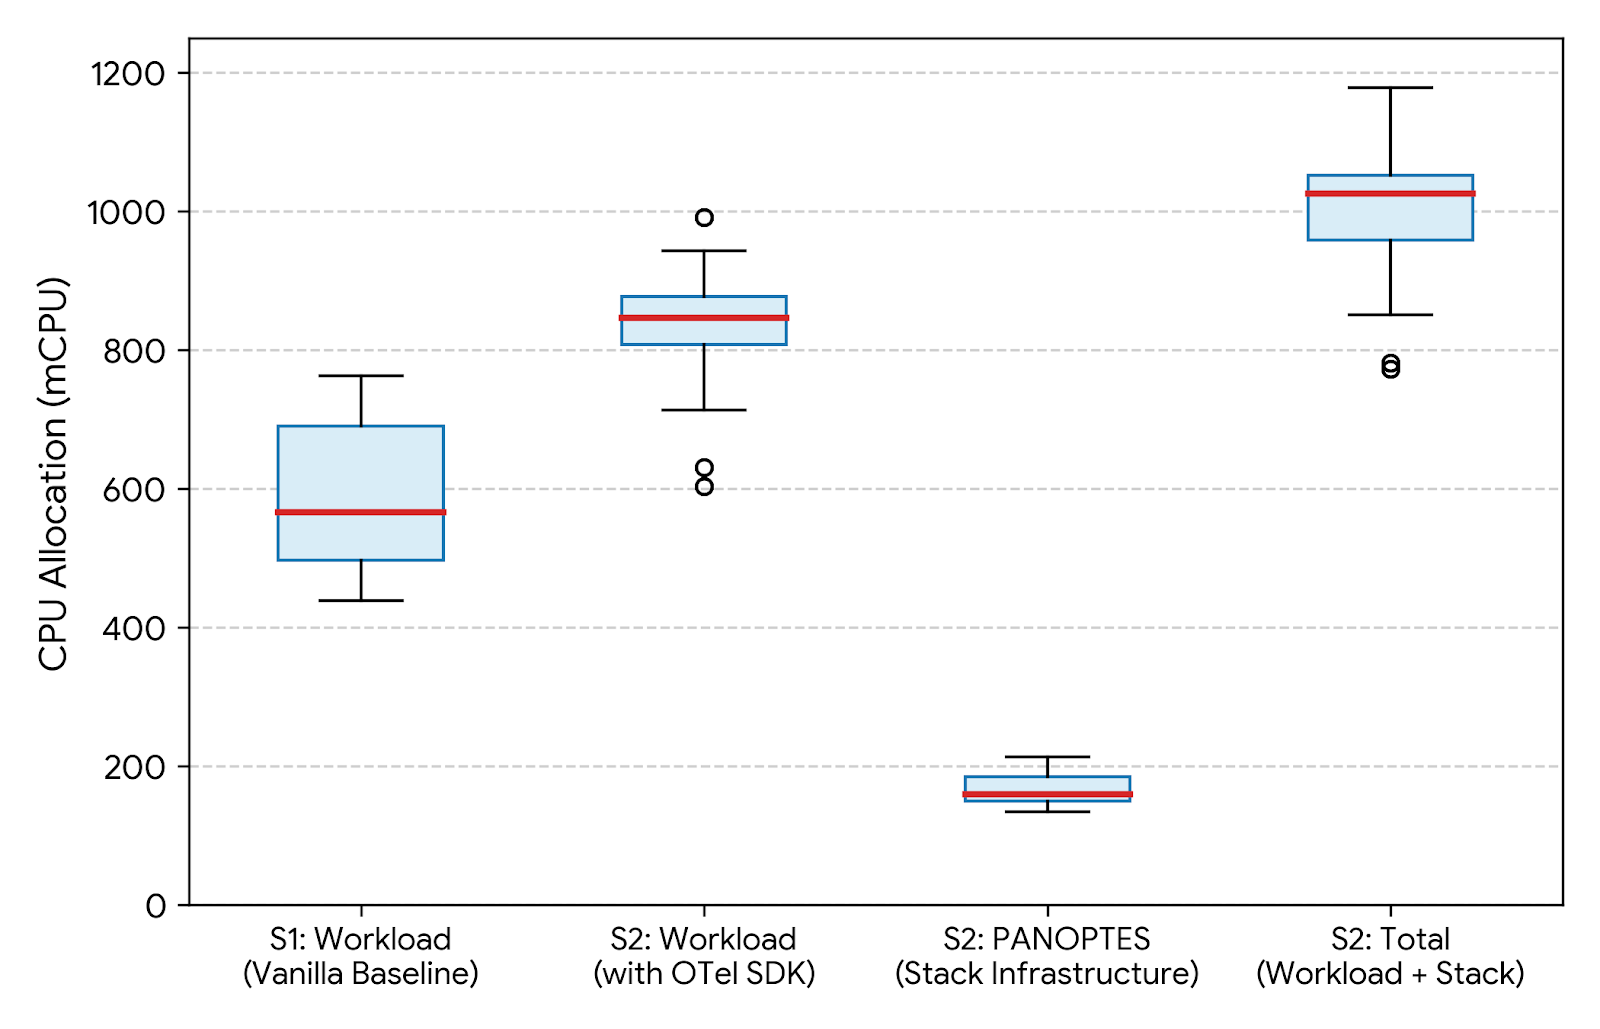
\includegraphics[width=0.75\textwidth]{images/results/scenario2_cpu_overhead.png}
    \caption{Steady-state CPU allocation distributions across Scenarios 1 and 2 ($N=30$).}
    \label{fig:scenario2_cpu_overhead}
\end{figure}

\begin{figure}[htbp]
    \centering
    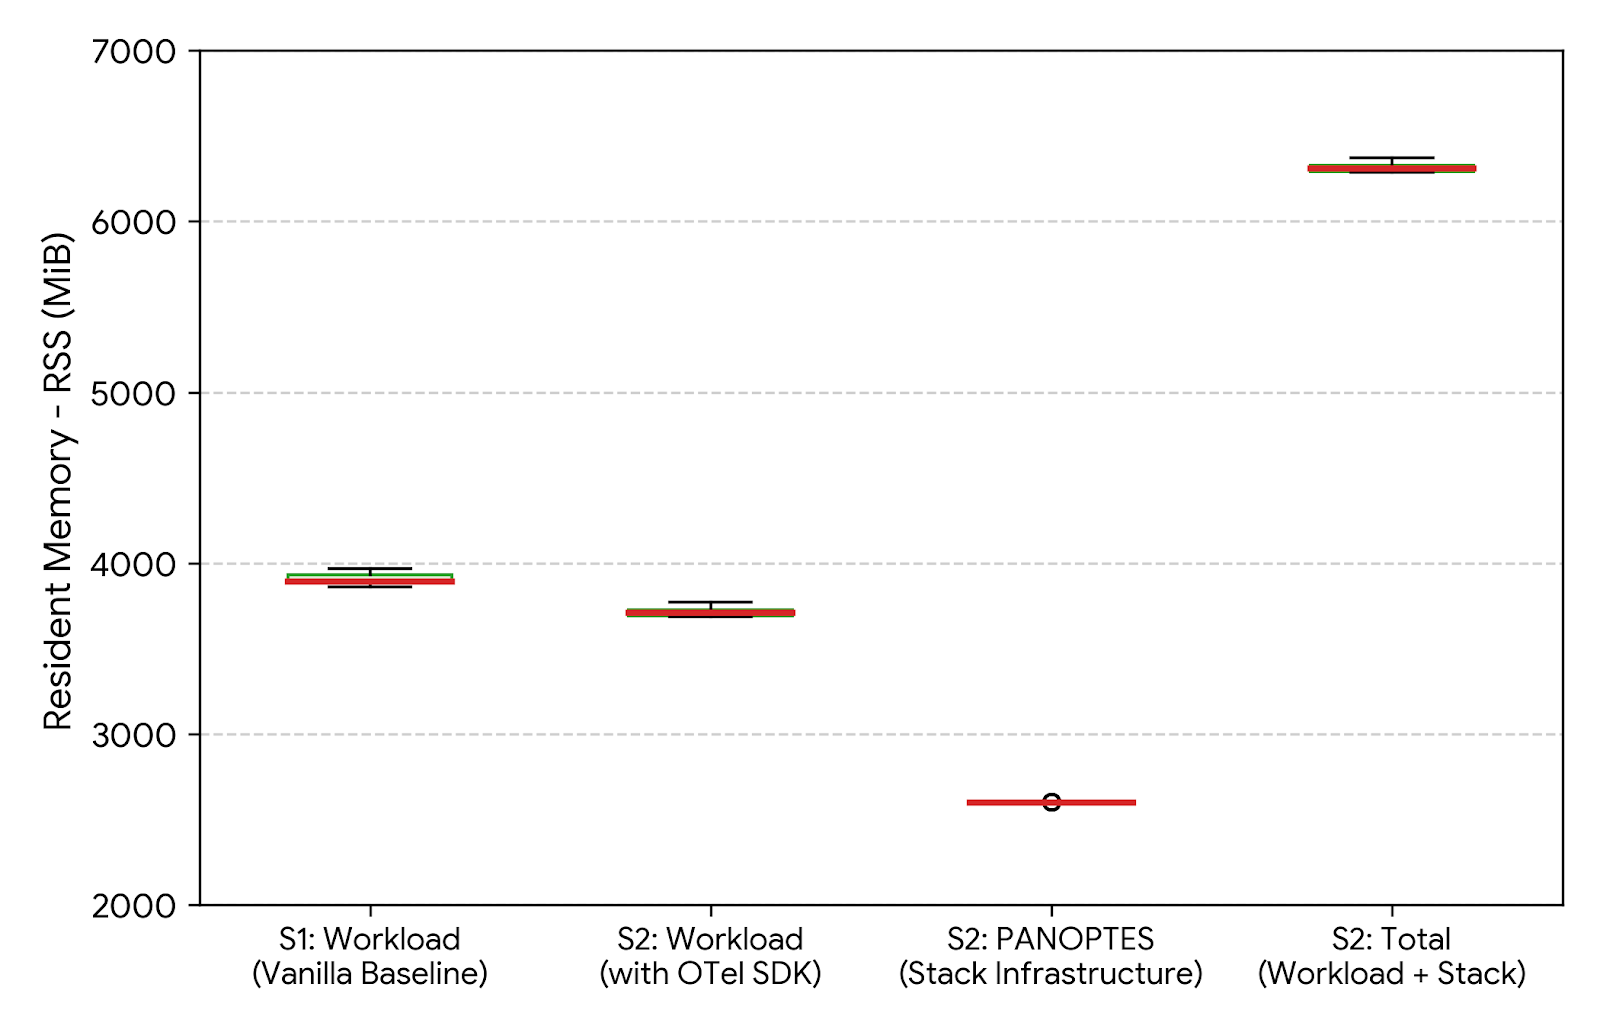
\includegraphics[width=0.75\textwidth]{images/results/scenario2_memory_overhead.png}
    \caption{Steady-state resident memory (RSS) distributions across Scenarios 1 and 2 ($N=30$).}
    \label{fig:scenario2_memory_overhead}
\end{figure}

A Shapiro-Wilk test confirmed non-normality across all metric distributions ($p < 0.05$). A two-sided Mann-Whitney $U$ test comparing total cluster demand between Scenario~1 and Scenario~2 confirmed statistically significant deltas for both CPU ($U = 0.0, \; p = 2.89 \times 10^{-11}$) and resident memory ($U = 0.0, \; p = 2.84 \times 10^{-11}$), validating the static baseline separation required to evaluate hypothesis $H_{1,3}$.